\begin{comment}
- Motivation --where are we going (end goal)
- Brief explanation between IoT and WoT
- Introduce FESTO water supply unit as example
- Scope of thesis


The key to remember is: Each device forms a web of semantic data, which can be queried with semantic web technology (like SPARQL).
\end{comment}




\chapter{Introduction}

Presently the Internet of Things (IoT) is a disjointed jumble of platforms, services, and \textit{Things}. Things include physical devices, such as sensors or actuators, applications, or even abstract concepts. In 2017 there were an estimated 450 IoT platform providers, including the Amazon AWS IoT and Microsoft's Azure IoT suite--that is a 25\% increase from 2016. 32\%  business-oriented platforms were intended for manufacturing/industrial services\cite{Williams.2017}. The seamless integration of wireless sensor networks and the IoT has enormous potential for industry and is a central pillar of the next industrial revolution, Industry 4.0.\cite{wang2016implementing}




\section{A Case for the Web of Things}

The options available for a business looking to integrate a factory into the IoT are overwhelming. There are thousands of devices on the market, hundreds of platforms, and dozens of protocols, just to name a few aspects to consider. Figure \ref{fig:IoT-landscape} shows some of the available options on the 2016 IoT market. This landscape is extraordinary diverse and disjointed.

\change{cite this correctly?}
\begin{figure}[th]
\centering
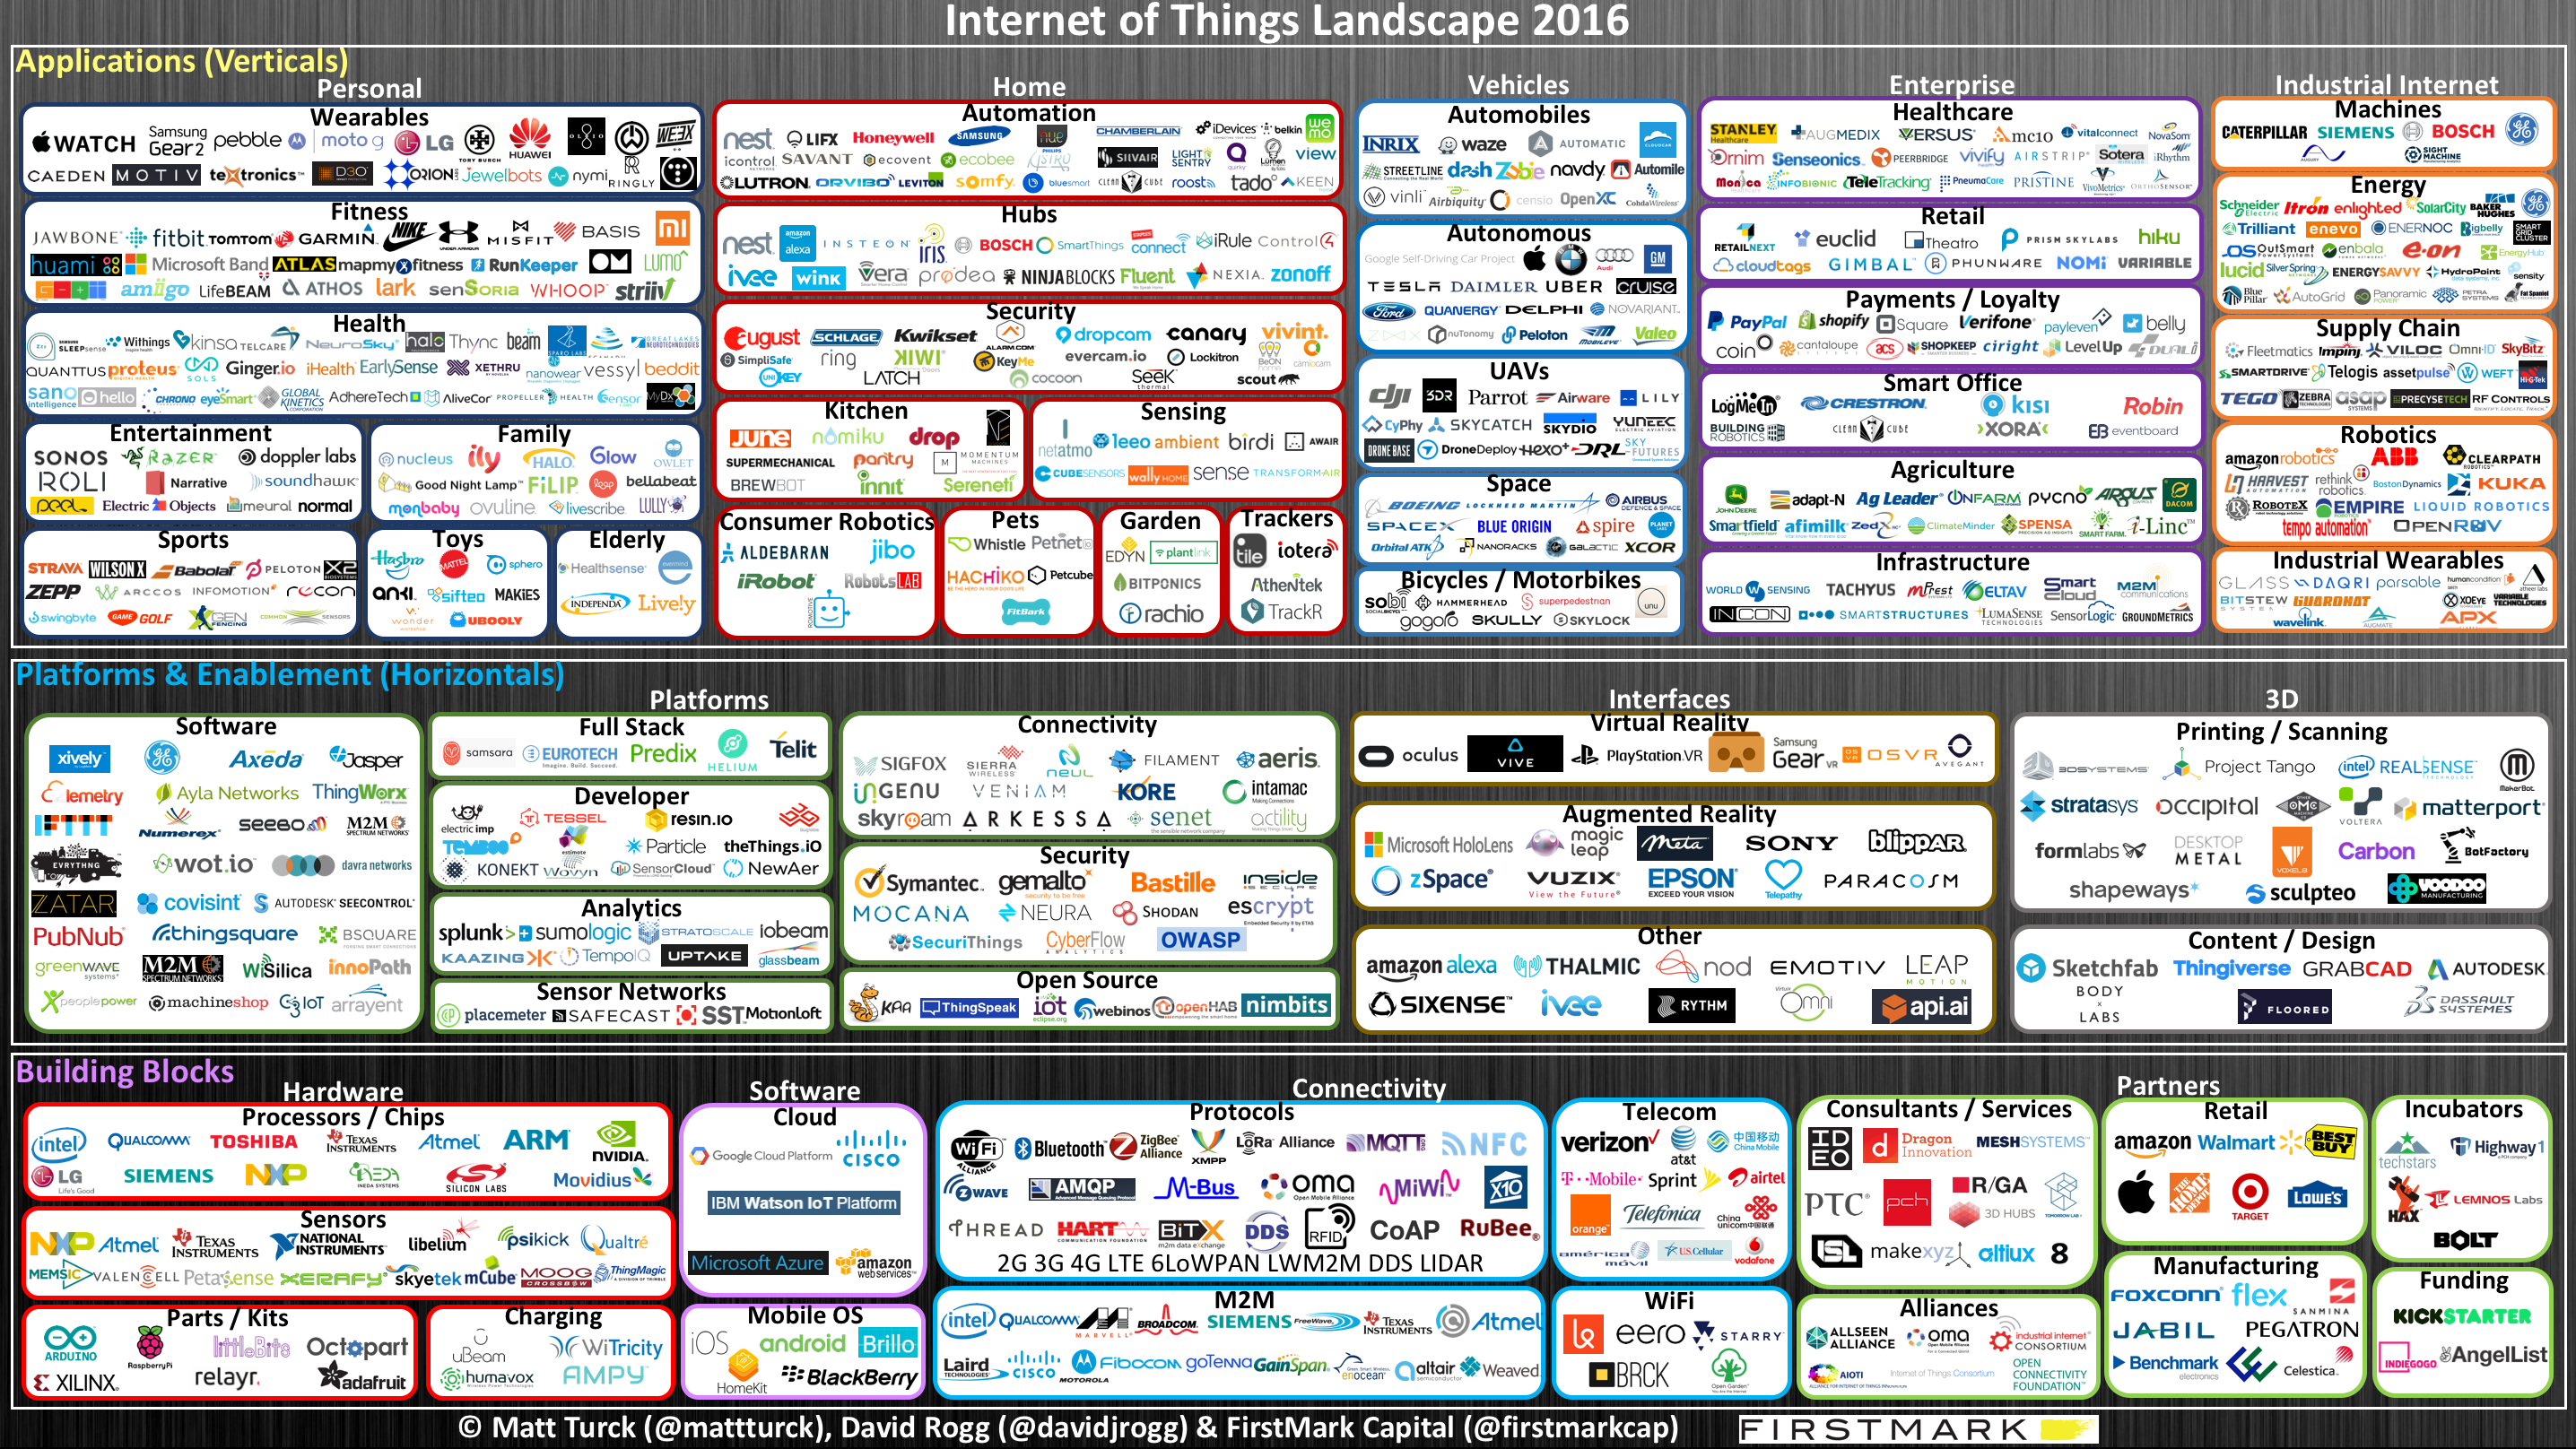
\includegraphics[width=\textwidth]{Figures/IoT-landscape}
\caption[Platforms and Options for the IoT in 2016]{An overwhelming amount of options for consumers and businesses. Source: Matt Turck}
\label{fig:IoT-landscape}
\footnote{http://mattturck.com/2016-iot-landscape/}
\end{figure}


The early Internet was likewise disjointed; accessing files on other computers was often tedious. Each computer connected to the network had a different set of applications, with which users had to be familiar. To counter this Tim Berners Lee invented the Web: the interconnected web of documents accessible in the same way from every computer. The Web revolutionized the way \textit{humans} access documents.


Analogous to the way humans are able to easily access documents all over the world thanks to the Web, so must machines be able to access \textit{data} across devices. However, the autonomous communication and configuration between Things is only possible, when those Things share common information models and implement the same protocols. One proposed approach to this problem reuses established Web technologies, like Semantic Web technology to serve as a common ground. This approach is called the \textit{Web of Things} (WoT). In a sentence its goal is to create a semantic web of data, in which each Thing is represented by a Web resource, which can be queried, much like a database. For this the World Wide Web Consortium (W3C) created a Web of Things Working Group and Interest Group, which together should build the stack for the Web of Things. \cite{.13Nov17}



\section{Motivation -- A Simple Business Case}
To understand the problem at hand, let us first consider the following example. Suppose we are residents of the city of the city of Musterberg, which is planning a cutting-edge water reclamation facility. It should be fully automated and connected to the Internet, so that the reclamation processes can be monitored from afar. This means each sensor and actuator needs a digital representation, which may be stored on one microcontroller.

The city council hires an engineer, Tricia, who must install and configure thousands of sensors and actuators. Aside from the physical configuration, Tricia has to create a distributed system, which could take years. With current technology Tricia would have to configure each device separately and create use cases for interaction patterns. That means, she has to tell devices, with whom they should communicate, what their responsibilities are, and what physical units they are working with.

In the IoT's current state it would require several years of manpower to set up this network and finally would yield a rigid network structure, in which (geographically) mobile Things cannot be easily integrated and additional use cases cannot be easily amended to the system.

Tricia has a deadline of 18 months--Musterberg is experiencing a population boom and the old reclamation facility is projected to not be able to keep up with the demand in within a year and a half. So Tricia has a few options: (1) hire an army of engineers and hope that will solve the problem, (2) use an established IoT platform.

If she (1) hires a large team of engineers Tricia will face the challenge of leading the team, and will certainly require a larger budget, which may not be available. Aside from that, throwing manpower at a problem this complex doesn't always help\footnote{Brook's Law: adding human resources to a late project will make it later.}. If she chooses to (2) use an established IoT platform, she will still likely require additional engineers and have the problem of researching, which platforms provide the services she actually requires. Additionally, most platforms have dubious data policies and confusing pricing schemes. Most platforms won't support the wide range of hardware that the reclamation facility will require, which means multiple platforms may be necessary. This adds the caveat, that they might not be compatible with each other and they also require different programming. This compatibility is referred to as interoperability and is a central challenge the IoT faces.

\begin{comment}


This example shows several of the main challenges the IoT is currently facing:
\begin{itemize}
    \item The difficulty of integrating heterogeneous hardware, this is referred to as interoperability.
    \item The challenge of picking an IoT platform or of using multiple platforms for one system.
    \item The issue of configuring a larger network, so that the system can be running as fast as possible.
    \item Standardization.
\end{itemize}

\change{merge together above and below paragraph}
\end{comment}

The goal of this thesis is to help Tricia by providing two discovery algorithms. One works in a centralized fashion, the other distributed. These algorithms find relevant partners for Things in their network with minimal human interaction. In order to provide proof of concept this work will benchmark the discovery algorithms on a miniature water supply unit from FESTO, which has been outfitted with Web of Things devices. The FESTO device serves as a minimum model for the water reclamation facility.


\section{Contributions}
This work starts by providing a brief background of the technology needed to realize a Web of Things. The focus for this being the importance of Semantic Web technology such as RDF, SPARQL, and the Thing Description.

In the next section the theory behind the three implemented algorithms will be discussed. This includes the REDD algorithm, which is a part of the centralized discovery algorithm, the centralized discovery algorithm itself, and the decentralized discovery algorithm.

After understanding the functionality of the algorithms, the next section will discuss the experimental setup and how the algorithms were evaluated. We will demonstrate the feasibility of discovery algorithms using only established web technology. Here we will also discuss the shortcomings of these algorithms.

This work will then conclude and  give an outlook for semantic discovery in the context of the Web of Things.
